\section*{Estacionaria como superposición de propagantes}

\item 
\begin{minipage}[t][2cm]{0.6\textwidth}
Una cuerda de longitud $L = \SI{0.6}{\metre}$, fija en sus dos extremos, oscila en uno de sus modos normales.
La velocidad de propagación de las ondas en dicha cuerda es \(v = \SI{80}{\metre\over\second}\).
En el momento que presenta su máxima amplitud pico a pico ésta es de \SI{8}{\milli\metre}.
\end{minipage}
\begin{minipage}[c][0.8cm][t]{0.34\textwidth}
	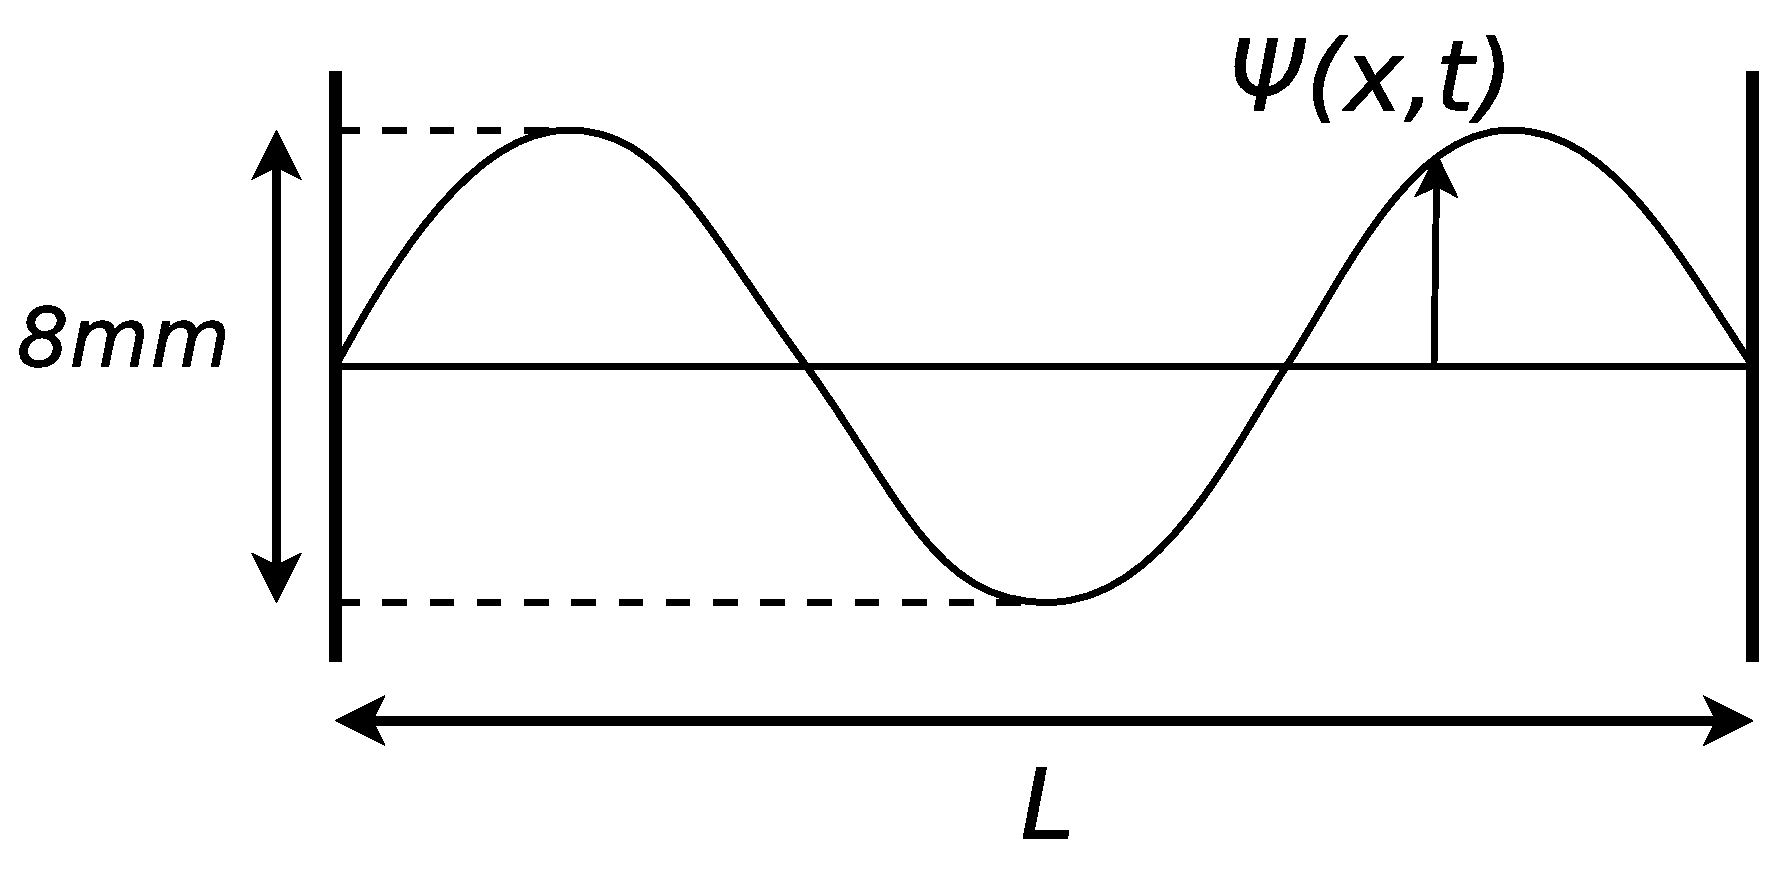
\includegraphics[width=\textwidth]{ej1-32}
\end{minipage}
\begin{enumerate}
	\item Escribir $\psi(x,t)$, sabiendo que $\psi(x,0) = 0\;\forall x$, y que $\dot{\psi}(L/2,0) > 0$.
	\item Hallar las ondas propagantes $\psi_+$ y \(\psi_-\) tales que $\psi(x,t)$ sea una combinación lineal de éstas.
\end{enumerate}


\item 
\begin{minipage}[t][2.5cm]{0.6\textwidth}
Una cuerda de longitud $L = \SI{1}{\metre}$, con un extremo fijo y uno libre, oscila en uno de sus modos normales.
La velocidad de propagación de las ondas en dicha cuerda es \(v= \SI{80}{\metre\over\second}\).
En \(t = 0\) presenta su máxima amplitud pico a pico de \SI{8}{\milli\metre}, siendo $\psi(L,0) > 0$.
\end{minipage}
\begin{minipage}[c][0.2cm][t]{0.34\textwidth}
	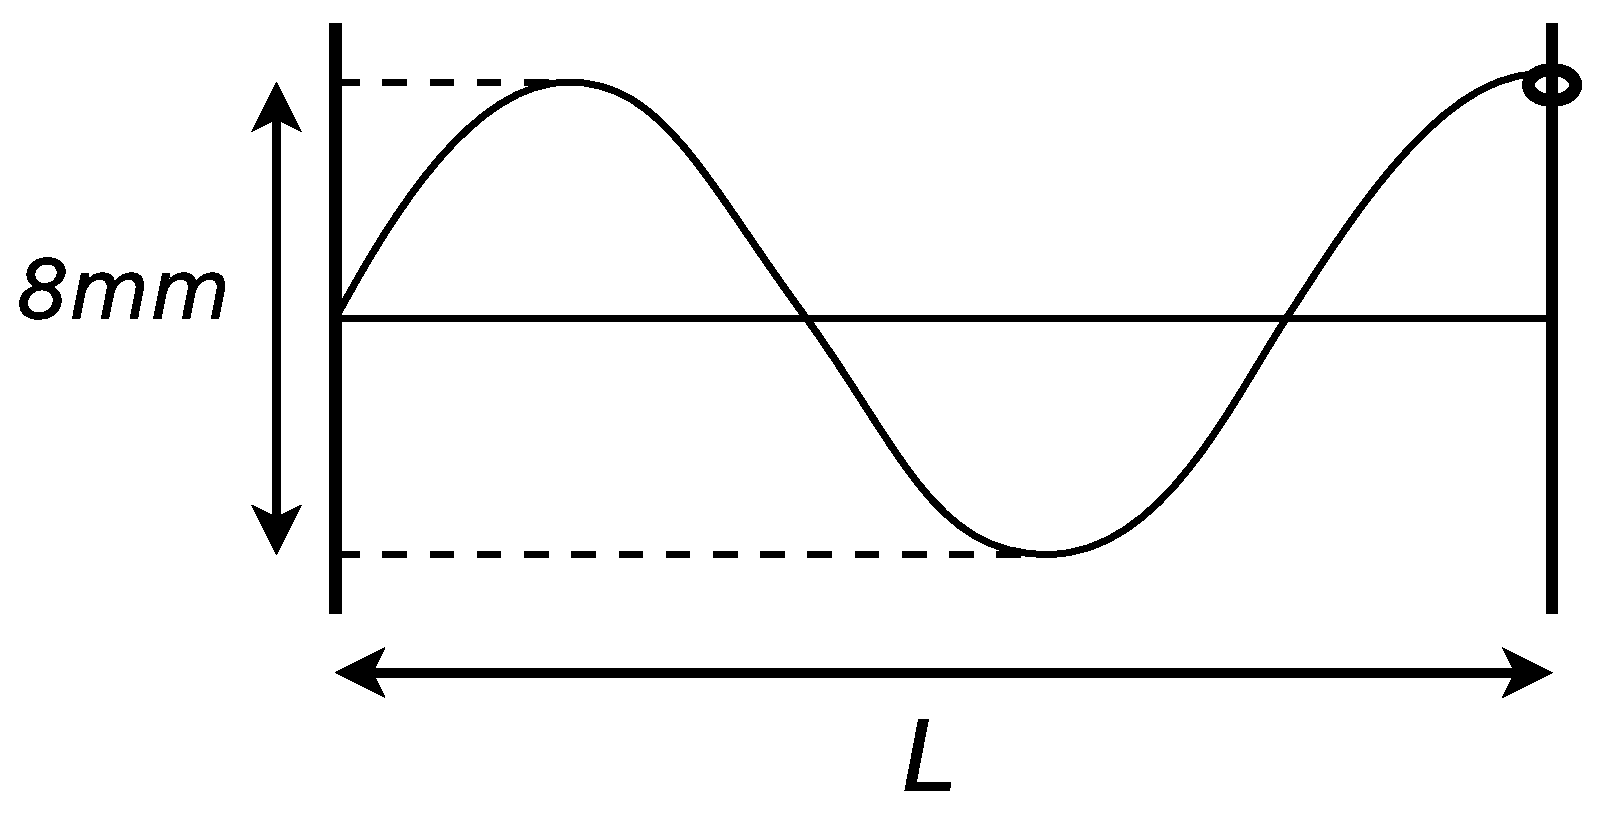
\includegraphics[width=\textwidth]{ej1-33}
\end{minipage}
\begin{enumerate}
	\item Resolver, para esta situación, todo lo pedido en el problema anterior. 
	\item Si ahora la cuerda está oscilando en un modo normal arbitrario $n$, con las mismas condiciones iniciales dadas arriba, repetir (a) (expresar en función de $n$).
\end{enumerate}
